\subsubsection{Hiện thực VNPay và bảo đảm ghi nhận một lần}
\label{sec:vnpay-implementation}
VnpayGateway chịu trách nhiệm cấu hình, build URL và QueryDr. Các hàm canonical/hmac/readCallback tách xử lý chữ ký khỏi nghiệp vụ. VnpayService.start/replay kiểm yêu cầu bắt đầu; ipn/returnUrl phân biệt hai kênh; apply ghi nhận kết quả; check điều phối đối soát theo yêu cầu. Frontend PaymentQr/VnpayPanel chỉ hiển thị và gọi API.

\paragraph{Xác minh trước khi ghi.}
Callback phải có dạng dữ liệu hợp lệ; canonical loại trường hash, sắp khóa và encode một lần; HMAC so bằng timingSafeEqual sau kiểm độ dài/định dạng. Chữ ký đúng vẫn phải kiểm merchant, txnRef, amount và mã trạng thái. Nhóm không xem chữ ký như mã hóa nội dung hoặc bằng chứng rằng đơn chắc chắn còn được phục vụ. QueryDr ký theo chuỗi trường của giao thức riêng, không dùng lại querystring của URL thanh toán.

\paragraph{Transaction và idempotency.}
apply khóa Order trước, đọc lại attempt và kiểm paidAt/khoản đã áp dụng. Với kết quả thành công, chỉ canFulfill khi đơn payable còn hạn, số tiền khớp và snapshot còn giữ. Payment, Order PAID, điểm và nhật ký cùng transaction; lỗi ở bước cộng điểm rollback cả settlement. Key của Payment theo txnRef, unique providerTxnNo và liên kết attempt là các lớp kiểm soát bổ sung; khóa Order điều phối cả hai attempt khác nhau của cùng đơn.

\paragraph{Không giữ khóa trong lúc chờ mạng.}
QueryDr thực hiện ngoài transaction, có timeout 8 giây. lastCheckedAt được cập nhật có điều kiện để hạn chế tra cứu dồn trong khoảng 15 giây; đây là điều tiết truy vấn, không phải kết quả tài chính. Khi response được xác minh, apply lấy khóa và kiểm lại điều kiện tại thời điểm ghi. HTTP 200 của endpoint IPN chỉ xác nhận HTTP có phản hồi; mã RspCode trong JSON mới là ACK nghiệp vụ, không thay thế trạng thái Order/Payment.

\begin{figure}[htbp]\centering
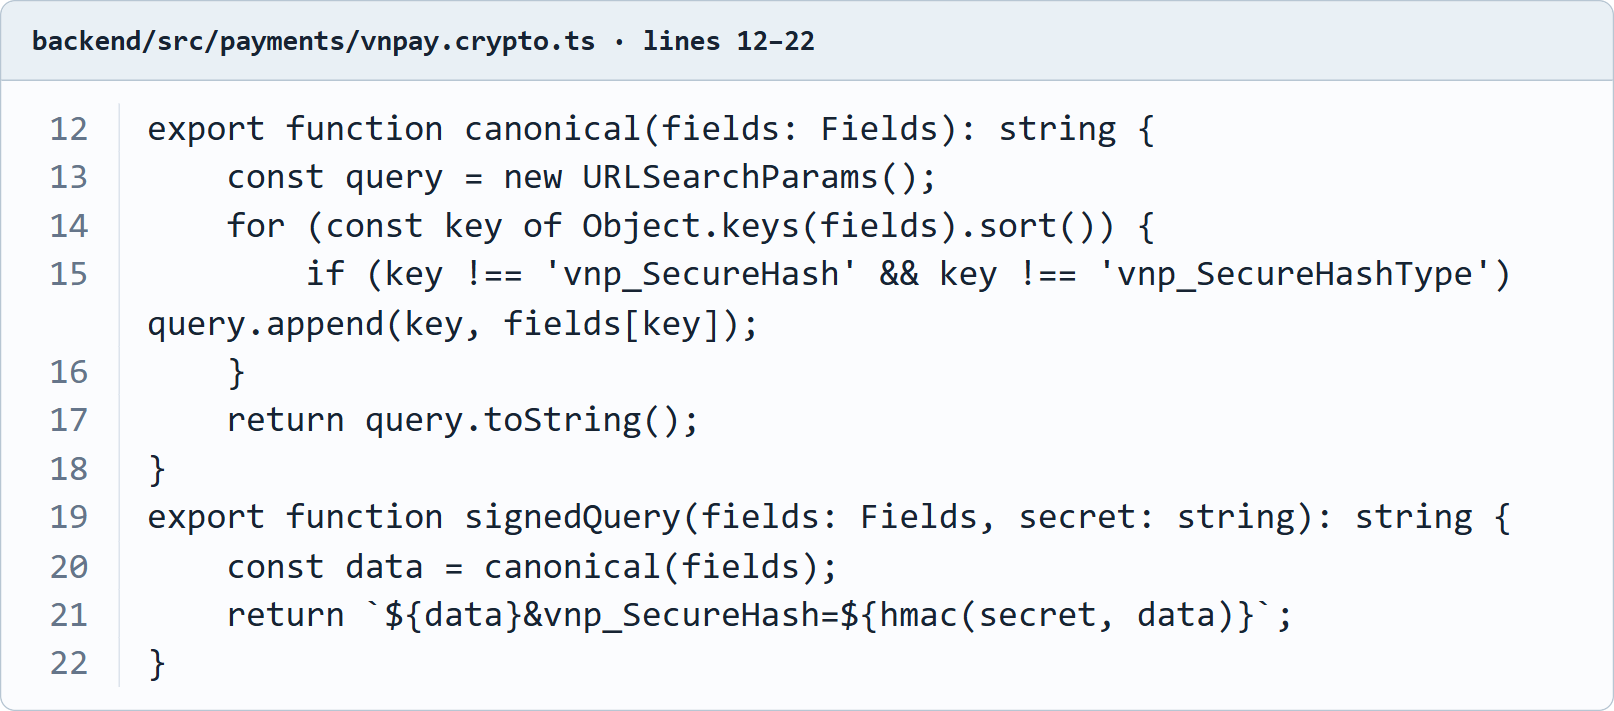
\includegraphics[width=.94\linewidth,height=.28\textheight,keepaspectratio]{assets/vnpay/code-canonical.png}
\caption{Chuẩn hóa tham số và ký URL trong vnpay.crypto.ts}
\vspace{4mm}
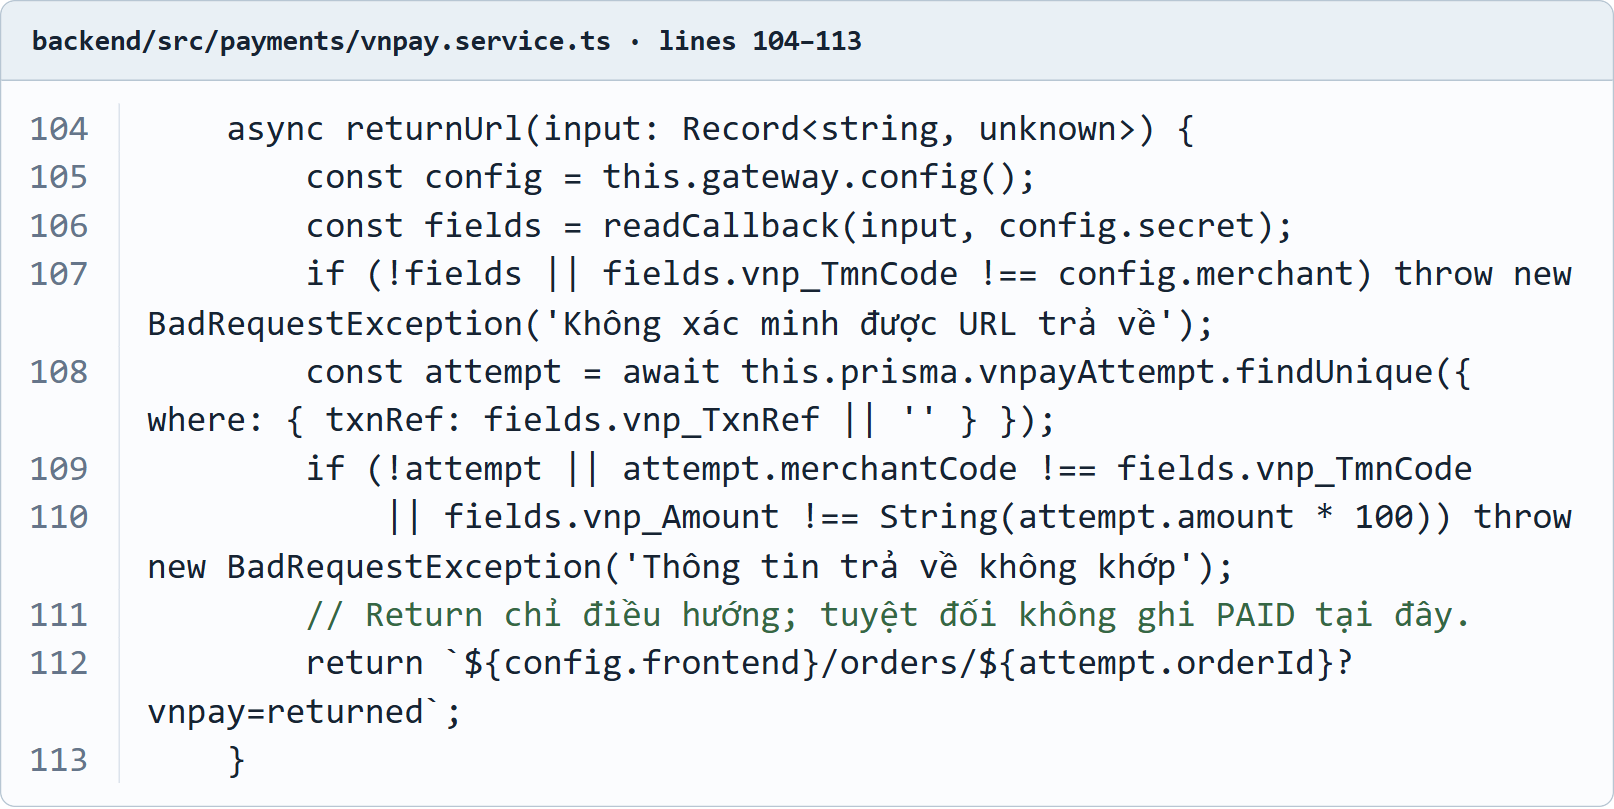
\includegraphics[width=.94\linewidth,height=.28\textheight,keepaspectratio]{assets/vnpay/code-return.png}
\caption{Return kiểm chứng dữ liệu rồi chỉ tạo đích chuyển hướng}
\end{figure}
\begin{figure}[htbp]\centering
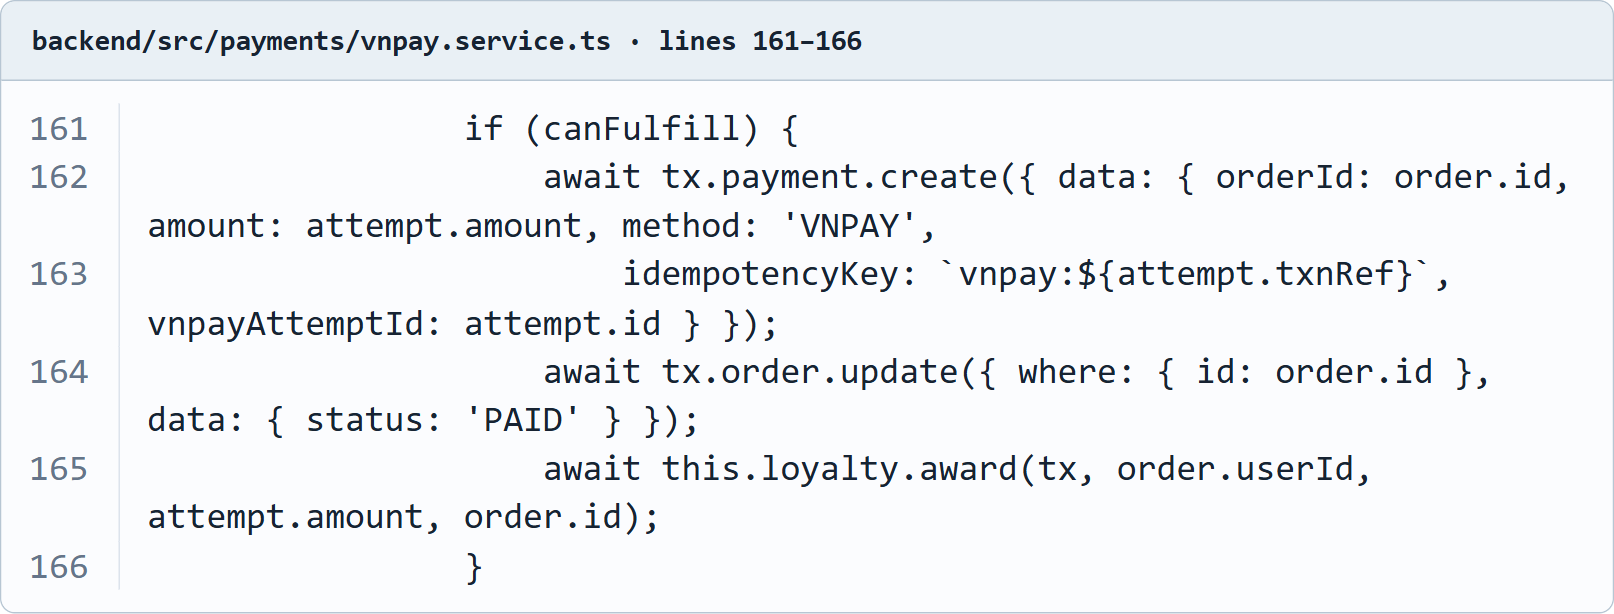
\includegraphics[width=.94\linewidth,height=.30\textheight,keepaspectratio]{assets/vnpay/code-settlement.png}
\caption{Nhánh canFulfill ghi Payment, PAID và điểm trong transaction apply}
\end{figure}
